\section{Projet}


La réflexion donc. La partie 2 est plus fun mais pour mieux cerner le
potentiel du projet, je vais détailler les fragments successifs à haute
valeur ajoutée d'une application de traitement de donnée moderne.  Ce
domaine applicatif est un leitmotiv des développements informatiques
actuels, centrés sur la data dont le flux s'accroît en permanence. Associé
à l'augmentation des capacités de stockage et de calcul des ordinateurs et
à leur accessibilité, il s'agit d'une formidable opportunité pour qui a les
connaissances requises.\newline \newline L'objectif dans les paragraphes
suivants est donc d'appréhender le pipeline que suit une donnée et de juger
des étapes sur lesquelles apporter une solution plus puissante et
innovante.\newline

%\begin{minipage}[c]{9cm}
\subsection{Data}
        Logiquement, le premier facteur clé est de la récupérer.
L'open-data est à la mode et les sources gratuites de qualité émergent.
QuanDL, twitter, marketdata, TrueFX, google finance, New-York Times\ldots proposent tous
une API dédiée à l'accès temps réel et gratuit de leurs données.
L'enjeu est donc d'être capable d'identifier les bonnes sources
d'information et de les exploiter.


\subsection{Formatage}
        La multiplication des sources a son revers: pertinence et fiabilité
non-systématique, quantité indigeste, doublons, synchronisation \ldots Un
premiet travail qui fait vivre nombre de sociétés de service est donc
d'appliquer une première transformation sur ce flux en le filtrant, nettoyant
et normalisant, puis en le stockant dans des infrastructures assurant
disponibilité rapide et permanente de quantités conséquentes et hautement
dynamiques. \newline
Cette étape permet déjà de mettre à la disposition de communautés
scientifiques compétentes de la matière sur laquelle produire des résultats
valorisant (monétairement, intellectuellement, voir plus (tips: le
médical)). Une perspective qui prend tout son sens
lorsque l'on sait que les scientifiques spécialisés déclarent consacrer
moins de la moitié de leur temps sur l'analyse proprement dire, du fait de
ce nettoyage chronophage qu'ils mènent eux-même, pour l'instant.
%\end{minipage}


%\newpage
%\begin{minipage}[c]{9cm}
\subsection{Enrichissement}
\textit{``any fool can know\ldots the point is to understand.'' - Albert
Einstein}\newline


Classiquement (quoique souvent amputé de l'étape précedente) tout ça est
tranquillement branché en direct sur les applications utilisatrices.
C'est gacher une opportunité! Toute cette quantité d'information peut
- doit - être passée à la moulinette des dernières techniques de data
mining, d'intelligence artificielle, d'algorithmes evolutionnistes,
\ldots pour extraire d'avantage que la signification brute. Pattern des
cours de bourse en regardant les années précédentes, prédiction de
comportement depuis tous les tweets, fiabilité des informations en comparant tous les
blogs, aide à la décision dans des systèmes à milliers de
variables.\newline
Avec cet enrichissement supplémentaire, on se fait les partenaires de
premier choix des applicatifs de traitement de données (soit une immense
majorité grandissante du secteur), des laboratoires
de recherche et d'autres institutions.


\subsection{Application}
        Arrive donc lesdites applications exploitant ce flux. Sans surprise la
tendance est aux cluster de bêtes de courses accessibles dans le cloud par
des clients légers. Et c'est pertinent: quoi de mieux que de simuler en 24s
10 années de stratégie algorithmique de trading depuis sa tablette qui
habituellement peine à décoder youtube. Avec la mise à disposition des
données, c'est le second atout à glisser dans les mains de thésards
chercheurs ou utilisateurs qui ne demandent pas mieux pour mettre en oeuvre
et rentabiliser leurs compétences.\newline
Pour prendre un exemple au coeur du sujet, le site quantopian.com qui
propose de simuler des stratégies de trading obtient un formidable retour
des communautés financières et scientifiques, qui toutefois doivent, pour
les meilleurs, construire eux mêmes depuis les simples cours des
données plus complexes. Ayant travaillé avec eux je sais que les
concepteurs sollicitent de nouvelles sources de data plus sophistiquées.


\subsection{Visualisation}

  Si on a bien travaillé jusqu'ici, on obtient de beaux résultats
tout neufs (hum au hasard, un portefeuille d'action qui performe à
43\%). Mieux vaut donc les voir.
L'enjeu est d'acquérir une véritable compréhension des problèmes
complexes étudiés et des résultats, afin d'enrichir la réflexion
et d'inférer efficacement sur la suite des évènements (avoir réussi
à analyser les liens sociaux de facebook et ne pas pouvoir se dépétrer de l'immonde
graphique qu'a pondu l'algorithme est sans doute frustrant).\newline
Coup de chance, l'avènement de l'ère de la data a poussé de nombreux
développeurs à créer des outils de visualisation qui explosent aujourd'hui
avec l'arrivée du HTML5 et de l'omniprésence du javascript.\newline
A cela s'ajoute l'esthétisme dont l'intérêt en terme de communication et de
diffusion n'est plus franchement à démontrer, pas plus qu'en matière
d'ergonomie.\newline
Pour les sceptiques: http://orbifold.net/html5/ et www.d3js.org

\begin{figure}[H]
  \begin{center}
     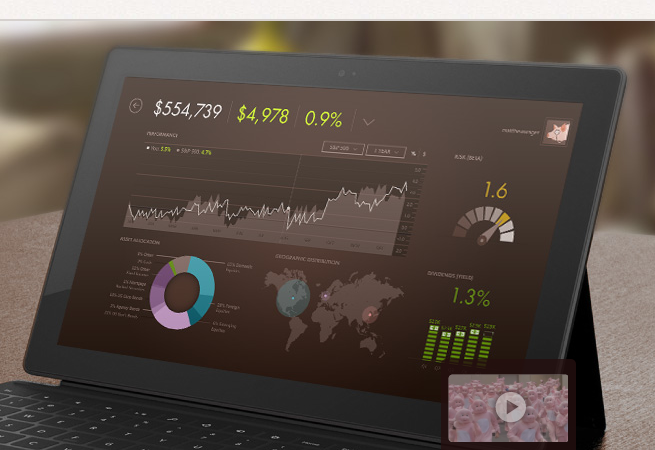
\includegraphics[scale=0.3]{images/sigpig.png}
    \end{center}
    \caption{portfolio visualization}
    \label{fig:viz}
\end{figure}


%\begin{minipage}[c]{9cm}
\subsection{Communauté}
        Je viens de parler de diffusion et j'ai évoqué deux fois la mise à
disposition des puissances processeurs et des capacités de stockage. L'idée en
effet est d'impliquer les communautés étudiantes, open-sources,
passionnées\ldots Pourquoi? Parce que les meilleurs cours de la planète
sont suivis gratuitement sur la base du volontariat par des millions
d'étudiants, que l'émulsion intellectuelle sur Quantopian.com est méchamment
productive, que les projets open-source permettent de faire partir ses codes
sur la base des meilleurs talents informatiques, que tous les jours les
meilleurs statisticiens partagent leurs connaisances sur r-bloggers.com. Et
parce que quand on est patron on aime avoir une équipe internationale de
milliers de développeurs qui ne demandent pas d'autre salaire qu'un projet
passionnant.


\subsection{Self-amélioration}
        Et voilà qui nous amène au dernier point du process. Le travail de
ces communautés, efficace grace aux outils cités et à la
collaboration, doit être réinjecté dans ces fameux outils , qui d'eux même s'amélioreront en
bouclant l'analyse!\newline
\newline
%\end{minipage}


Ce qu'il faut retenir : Pendant que la guerre fait rage sur les applicatifs
et services informatiques, allons nous pluger en amont en interceptant,
enrichissant, et refourguant de la donnée évoluée, et en aval pour
valoriser leurs résultats. Et enfin impliquons les communautés open-source
pour diminuer les frais et augmenter l'intelligence et la créativité des
solutions.\newline
Et tant qu'on y est développons le tout sur un système de trading que j'ai
déjà écrit qui servira de fer de lance communiquant et crédible, et
produira les bonus de début, milieu et fin de mois.
\newpage




% section Projet (end)
